
\subsection{Alinhamento da ferramenta com a porta de acoplamento}
\label{subsec_cap4_alinhamento}

Esta subseção apresenta o alinhamento entre o eixo longitudinal da ferramenta do manipulador robótico e a normal da porta de acoplamento, ambas expressas no referencial $\{0\}$.
O alinhamento é avaliado por
(i) uma métrica angular,
(ii) o produto escalar entre vetores unitários,
(iii) a decomposição do produto escalar por eixo e
(iv) a coerência dessas métricas com o erro de posição do efetuador final em relação à referência gerada pela cinemática inversa.

% \subsubsection{Definições geométricas e normalização dos vetores}
% \label{subsubsec_cap4_alinhamento_definicoes}

% Sejam $\vec{e}_{\text{tool}}$ o vetor diretor associado ao eixo da ferramenta e $\vec{n}_{\text{porta}}$ o vetor normal da porta, ambos em $\{0\}$.
% Para evitar vieses quando os vetores não são fornecidos unitários, utiliza-se a versão normalizada, $\hat{\vec{e}}_{\text{tool}}$ e $\hat{\vec{n}}_{\text{porta}}$, obtida pela divisão de cada vetor por sua norma euclidiana.
% Dessa forma, as métricas de alinhamento dependem apenas da direção e não da magnitude numérica dos vetores.

\subsubsection{Ângulo de alinhamento}
\label{subsubsec_cap4_alinhamento_angulo}

O erro angular de alinhamento é definido como o ângulo entre o eixo longitudinal da ferramenta e a normal da porta de acoplamento, ambos expressos no referencial $\{0\}$.
Essa métrica permite interpretação direta em graus e fornece uma medida geométrica imediata e relevante para o acoplamento.

% A Figura~\ref{fig_cap4_alinhamento_MR} ilustra a definição geométrica adotada, destacando o eixo da ferramenta, o efetuador final e a normal da porta.
Na fase anterior ao início do modo operacional do \gls{mr} (até $t_\text{operacao}=466{,}26~\mathrm{s}$), o eixo da ferramenta permanece aproximadamente perpendicular à normal da porta, resultando em um ângulo próximo de $90^\circ$.
A partir do modo operacional, o manipulador passa a executar a manobra de alinhamento, reduzindo progressivamente o erro angular.
Valores mais próximos de $0^\circ$ indicam melhor alinhamento, pois representam maior colinearidade entre o eixo da ferramenta e a normal da porta.

% \begin{figure}[H]
% \centering
% 
\includegraphics[width=1.0\linewidth]{\detokenize{5 Resultados/Imagens/4 Alinhamento/Alinhamento 1 MR.png}}
% \caption{Definição geométrica dos eixos utilizados na avaliação de alinhamento: eixo da ferramenta e normal da porta de acoplamento, no referencial $\{0\}$.}
% \label{fig_cap4_alinhamento_MR}
% \end{figure}

A Figura~\ref{fig_cap4_alinhamento_angulo} apresenta a evolução temporal do ângulo de alinhamento.
Observa-se a transição do regime inicial, com ângulo próximo de $90^\circ$, para valores de poucos graus após $t_{\text{operacao}}$, atingindo $5{,}16^\circ$ no instante de acoplamento ($t_{\text{acopl}}=662{,}57~\mathrm{s}$) e $6{,}77^\circ$ no instante final ($t_f=900{,}00~\mathrm{s}$).

\begin{figure}[H]
\centering

\includegraphics[width=1.0\linewidth]{\detokenize{5 Resultados/Imagens/4 Alinhamento/Alinhamento 1 Angulo.png}}
\caption{Ângulo entre o eixo da ferramenta e a normal da porta, expresso no referencial $\{0\}$.}
\label{fig_cap4_alinhamento_angulo}
\end{figure}


\subsubsection{Componentes do eixo da ferramenta no referencial $\{0\}$}
\label{subsubsec_cap4_alinhamento_componentes_etool}

A decomposição do eixo unitário da ferramenta em componentes no referencial $\{0\}$ permite identificar quais direções cartesianas dominam a orientação da ferramenta ao longo da manobra, bem como localizar transientes associados à atuação do manipulador.
Essa análise complementa as métricas escalares (ângulo e produto escalar), pois explicita quais variações direcionais são responsáveis pelas mudanças observadas nessas grandezas.

A Figura~\ref{fig_cap4_alinhamento_eixo_ferramenta_xyz} apresenta a evolução temporal das componentes do vetor unitário $\vec{e}_{\text{tool}}$ em $\{0\}$.
Cada componente representa a projeção do eixo da ferramenta sobre o respectivo eixo cartesiano de $\{0\}$: valores próximos de $0$ indicam baixa contribuição daquela direção para a orientação instantânea, enquanto valores próximos de $1$ indicam alinhamento com o respectivo eixo.
Assim, o comportamento conjunto das três componentes descreve a rotação do eixo da ferramenta durante a fase de alinhamento.

\begin{figure}[H]
\centering

\includegraphics[width=1.0\linewidth]{\detokenize{5 Resultados/Imagens/4 Alinhamento/Alinhamento 2 Eixo xyz eef.png}}
\caption{Componentes do eixo unitário da ferramenta no referencial $\{0\}$ ao longo do tempo.}
\label{fig_cap4_alinhamento_eixo_ferramenta_xyz}
\end{figure}


\subsubsection{Produto escalar como métrica de colinearidade}
\label{subsubsec_cap4_alinhamento_produto_escalar}

O produto escalar, apresentado na Figura~\ref{fig_cap4_alinhamento_prod_escalar}, entre o eixo da ferramenta e o eixo da porta de acoplamento é empregado como métrica de colinearidade.
Valores próximos de $1$ indicam alinhamento direcional, enquanto valores negativos indicam orientação oposta.
Essa métrica complementa o ângulo por fornecer uma medida contínua no intervalo $[-1,1]$ e por refletir diretamente a projeção entre as direções.

\begin{figure}[H]
\centering
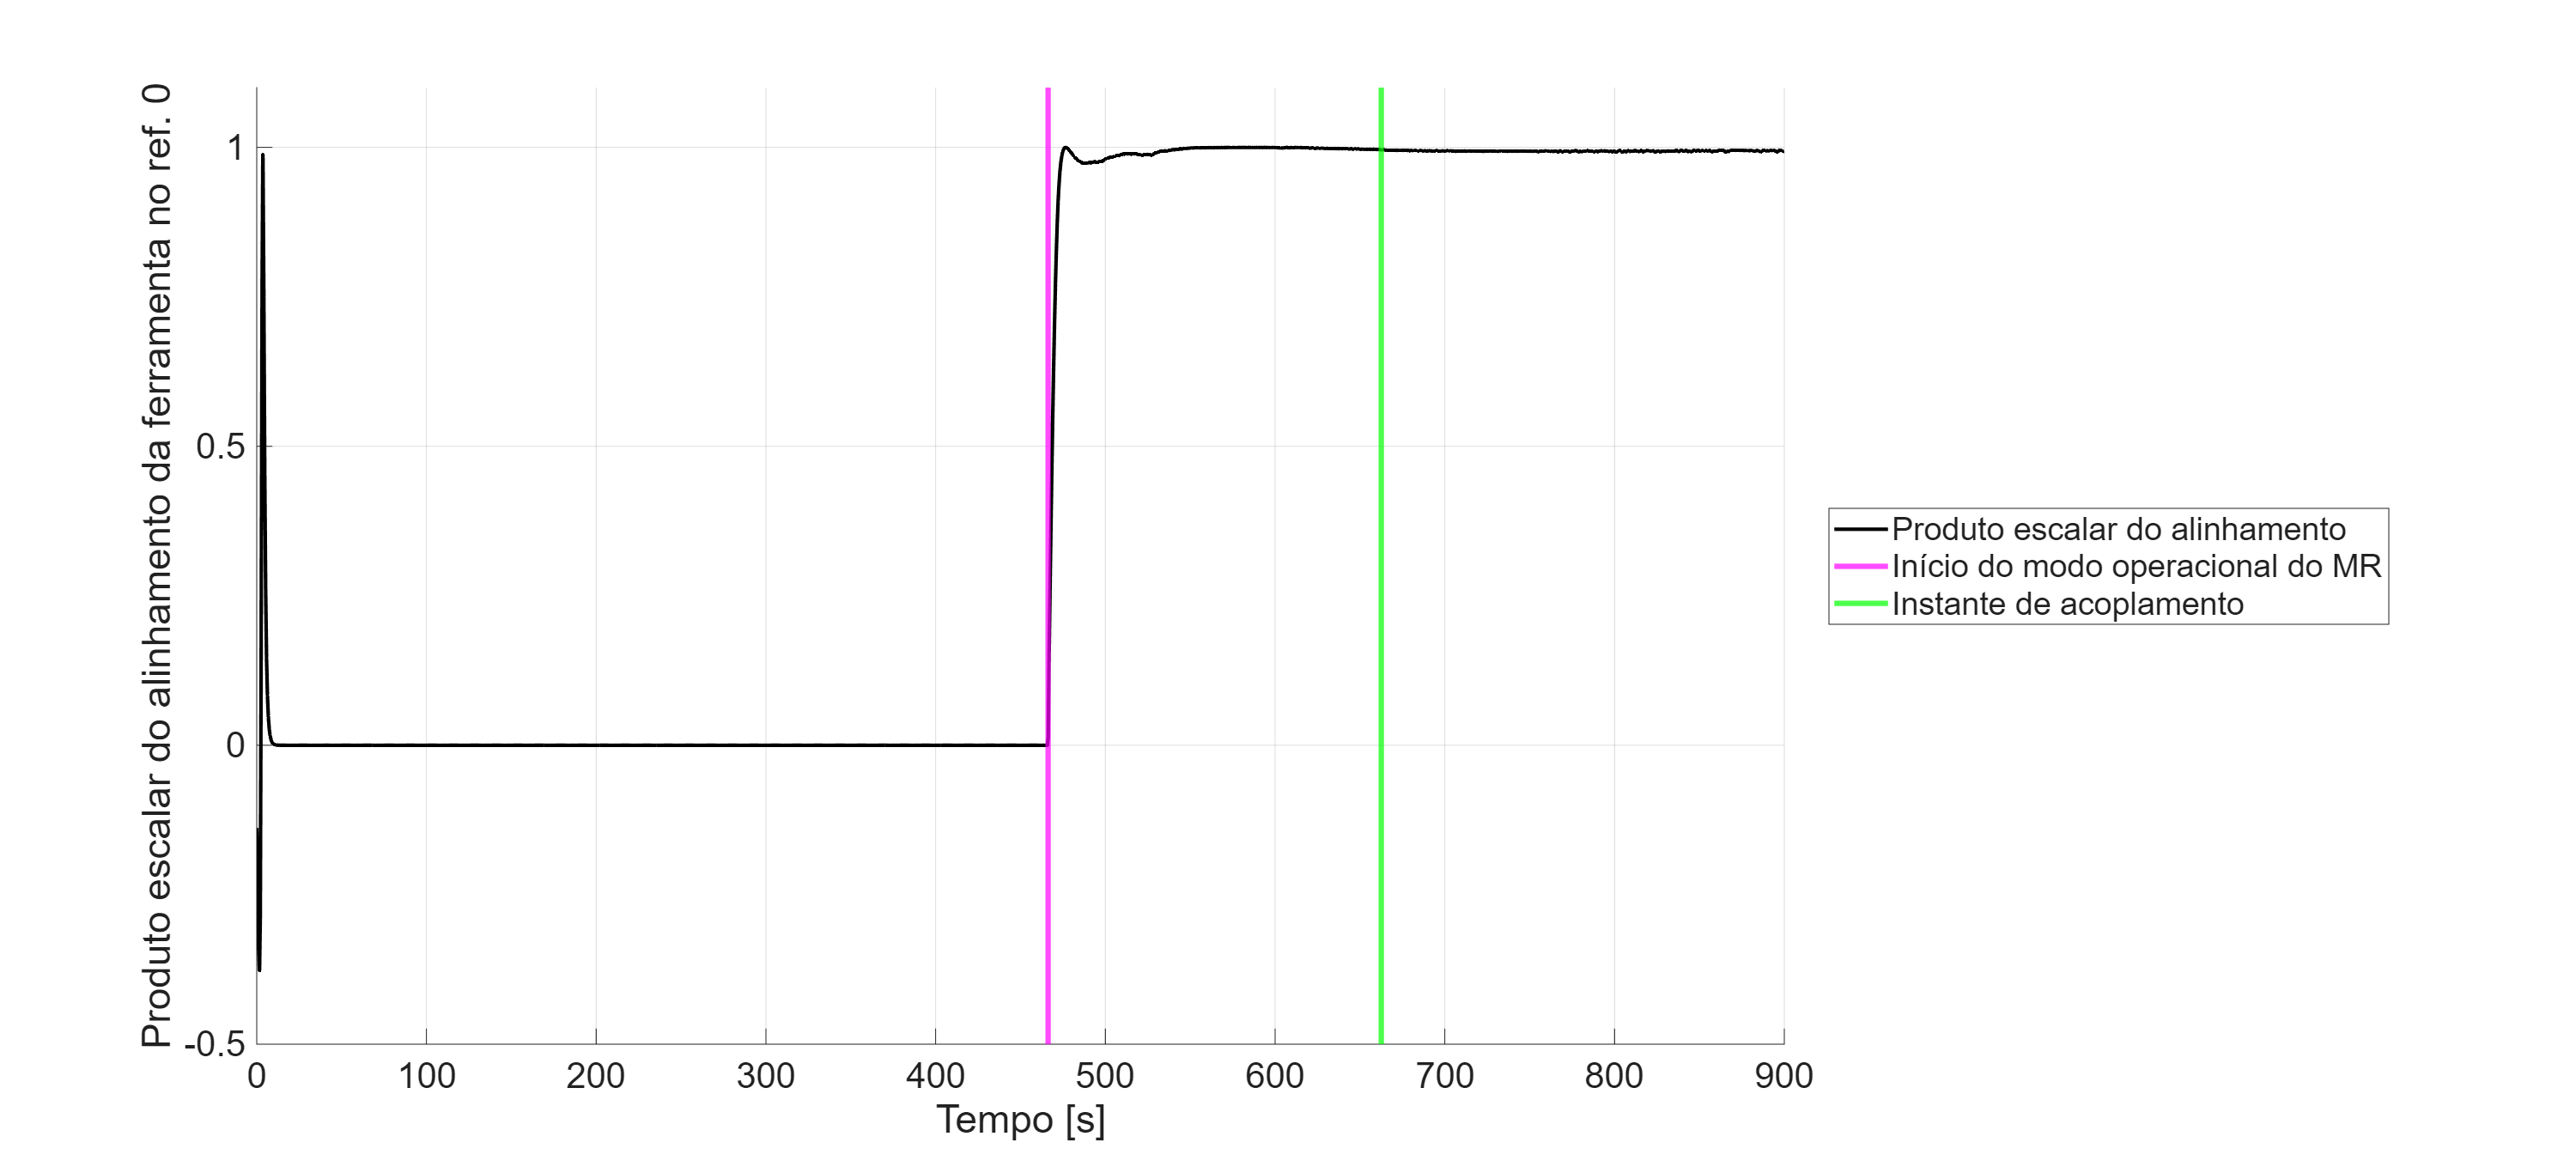
\includegraphics[width=1.0\linewidth]{5 Resultados/Imagens/4 Alinhamento/Alinhamento 3 Prod escalar.png}
\caption{Produto escalar entre o eixo unitário da ferramenta e a normal unitária da porta, expresso no referencial $\{0\}$.}
\label{fig_cap4_alinhamento_prod_escalar}
\end{figure}

\subsubsection{Decomposição do produto escalar por eixo}
\label{subsubsec_cap4_alinhamento_decomposicao_xyz}

Para identificar quais componentes no referencial $\{0\}$ contribuem para o alinhamento, o produto escalar é decomposto nas parcelas associadas às componentes $x$, $y$ e $z$ de $\{0\}$, conforme a Figura~\ref{fig_cap4_alinhamento_contribuicao_xyz}.
A soma das contribuições por eixo recupera o produto escalar total, permitindo verificar consistência interna e interpretar o papel relativo de cada direção no alinhamento resultante.

\begin{figure}[H]
\centering
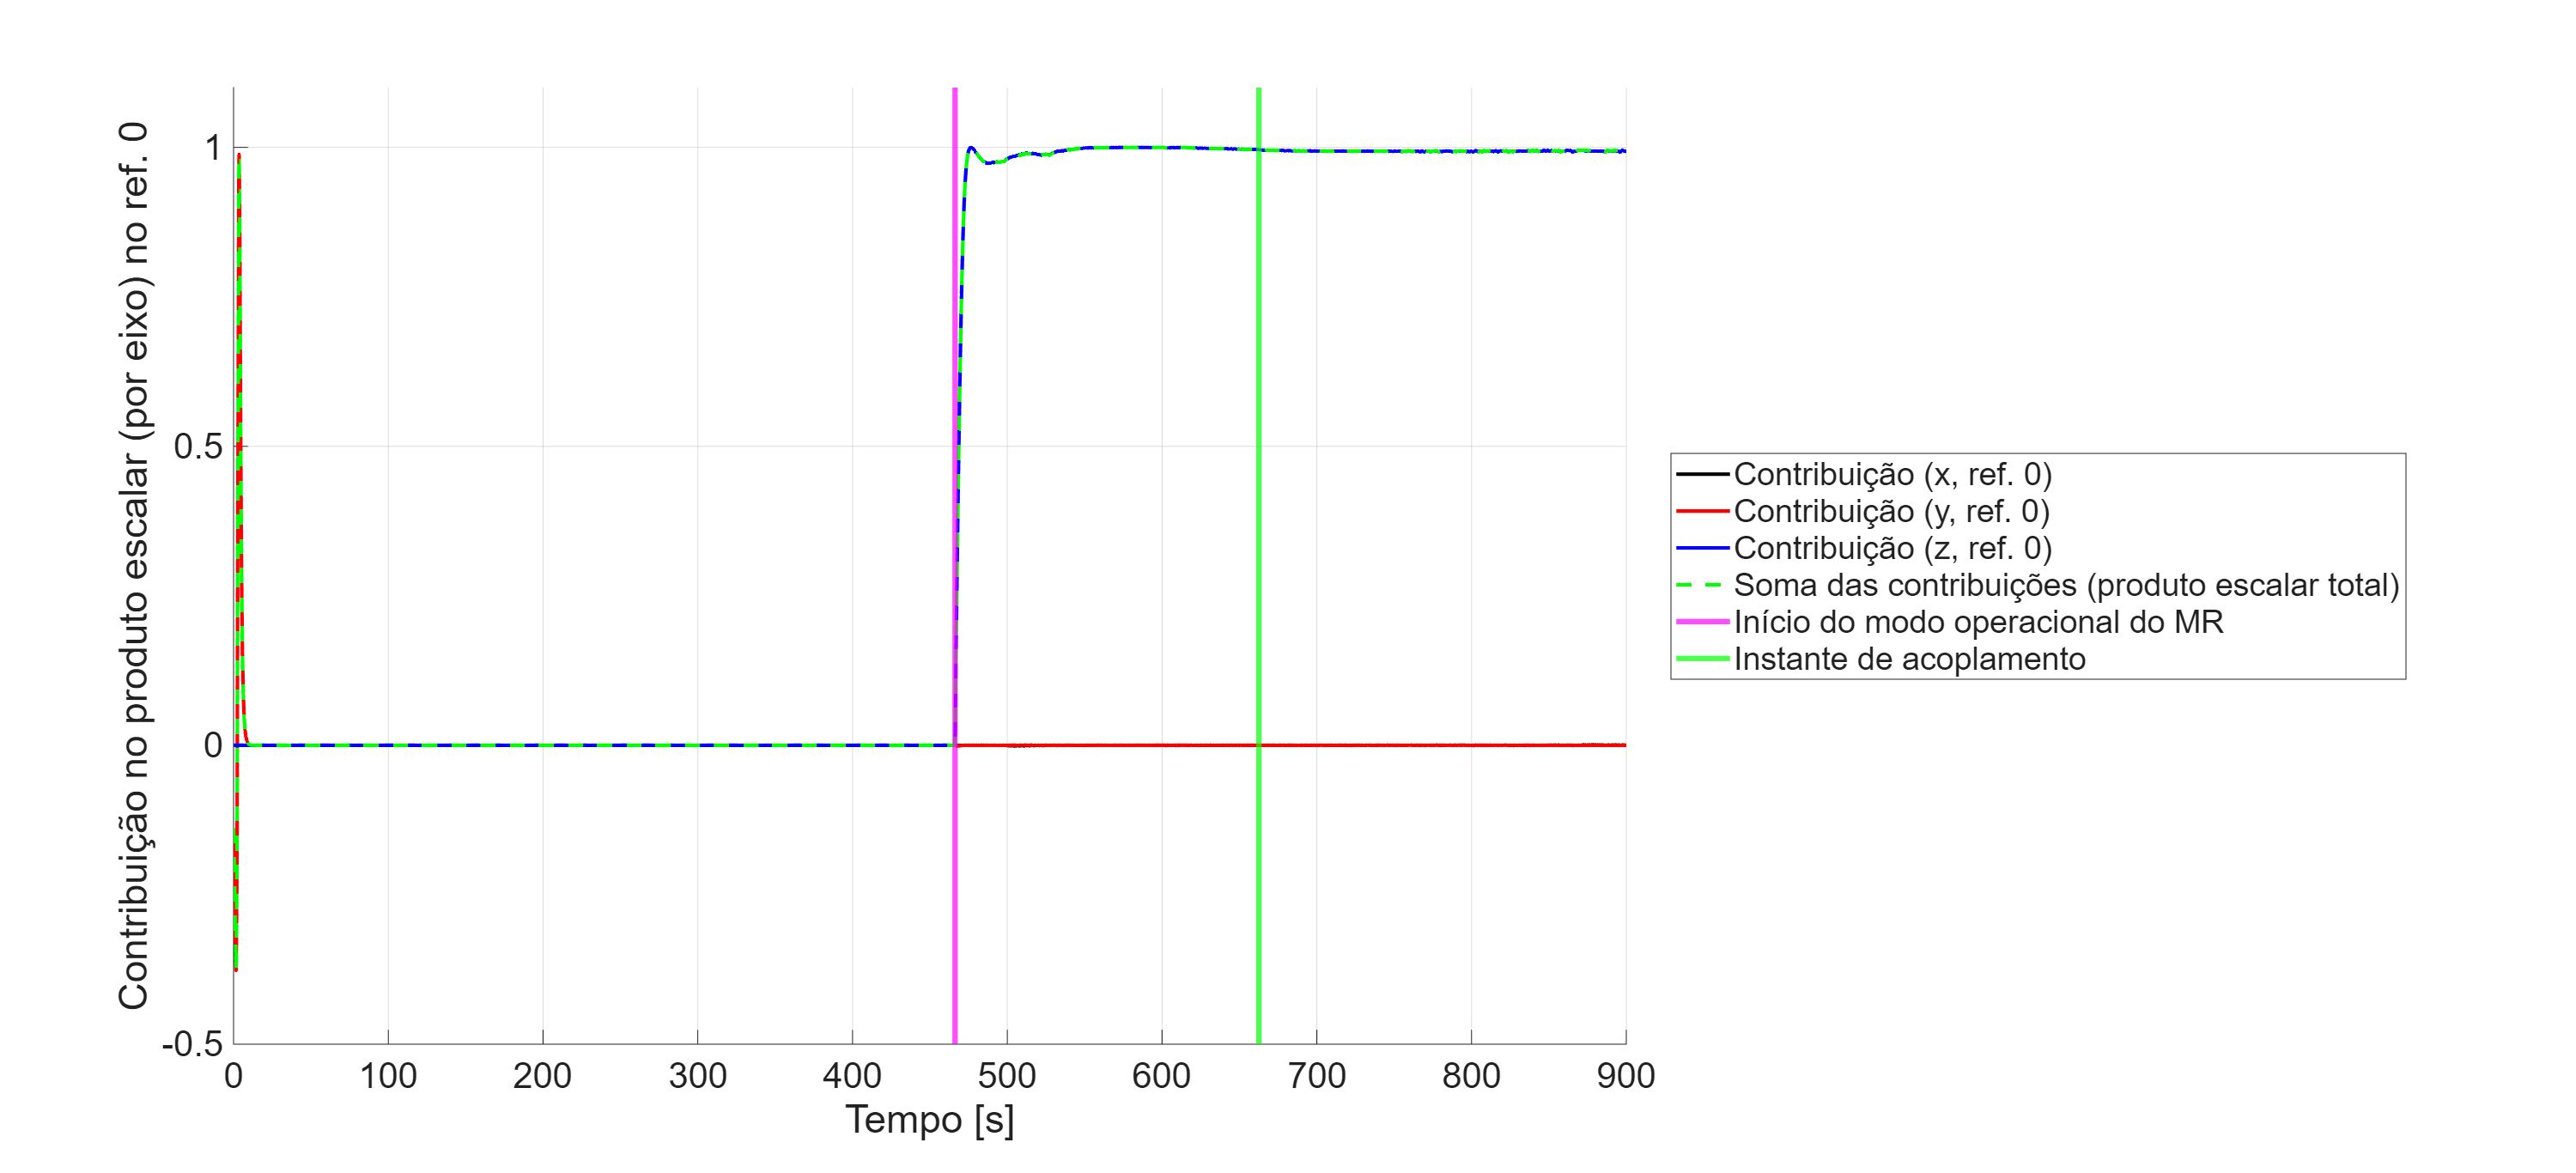
\includegraphics[width=1.0\linewidth]{5 Resultados/Imagens/4 Alinhamento/Alinhamento 4 Contribuicao por eixo.png}
\caption{Contribuições por eixo no produto escalar de alinhamento no referencial $\{0\}$ e sua soma.}
\label{fig_cap4_alinhamento_contribuicao_xyz}
\end{figure}



\subsubsection{Erro de posição da ferramenta durante o alinhamento}
\label{subsubsec_cap4_alinhamento_erro_posicao}

Em paralelo às métricas direcionais, avalia-se o erro de posição do efetuador final em relação à posição de referência fornecida pela cinemática inversa, ambas expressas no referencial $\{0\}$.
A análise contempla (i) a magnitude do erro e (ii) suas componentes cartesianas.
Essa verificação permite discutir se a convergência direcional (alinhamento) ocorre de forma compatível com a convergência translacional (aproximação) ao longo do intervalo operacional.

A Figura~\ref{fig_cap4_alinhamento_erro_posicao} reúne três subgráficos complementares.
O primeiro apresenta a magnitude do erro de posição, evidenciando decaimento progressivo durante a aproximação curta, até valores residuais baixos ao final do intervalo.
O segundo subgráfico apresenta as componentes cartesianas do erro em $\{0\}$, permitindo identificar quais direções dominam o erro translacional e verificar a redução simultânea em $x$, $y$ e $z$.
Por fim, o terceiro subgráfico aplica uma escala temporal ampliada no início da simulação, de modo a evidenciar o transiente inicial associado ao acionamento instantâneo das malhas de controle, à dinâmica do corpo rígido e ao processo de alinhamento de atitude do perseguidor.

\begin{figure}[H]
\centering

\includegraphics[width=1.0\linewidth]{\detokenize{5 Resultados/Imagens/4 Alinhamento/Alinhamento 5 Erro posicao eef.png}}
\caption{Erro de posição do efetuador final em relação à referência de cinemática inversa, expresso no referencial $\{0\}$: (a) magnitude, (b) componentes cartesianas e (c) destaque do transiente inicial.}
\label{fig_cap4_alinhamento_erro_posicao}
\end{figure}


\subsubsection{Instantes característicos e coerência entre métricas}
\label{subsubsec_cap4_alinhamento_eventos_coerencia}

Para contextualizar os resultados, são destacados os instantes característicos: início do modo operacional do manipulador ($t_{\text{operacao}}$) e instante de acoplamento ($t_{\text{acopl}}$).
A Tabela~\ref{tab_cap4_alinhamento_eventos} apresenta as métricas nesses instantes e no final da simulação, indicando a evolução conjunta do ângulo, do produto escalar e do erro de posição.

\begin{table}[H]
\centering
\caption{Métricas de alinhamento em instantes característicos.}
\label{tab_cap4_alinhamento_eventos}
\begin{tabularx}{\linewidth}{|
  >{\centering\arraybackslash}X|
  >{\centering\arraybackslash}X|
  >{\centering\arraybackslash}X|
  >{\centering\arraybackslash}X|
  >{\centering\arraybackslash}X|}
\hline
\textbf{Instante} &
\textbf{Tempo [s]} &
\textbf{Ângulo [${}^\circ$]} &
\textbf{Produto escalar [-]} &
\textbf{Erro de posição [m]} \\
\hhline{|=|=|=|=|=|}
Início do modo operacional do MR ($t_{\text{operacao}}$) & $466{,}26$ & $90{,}00$ & $0{,}0000$ & $1{,}3244$ \\
\hline
Acoplamento ($t_{\text{acopl}}$) & $662{,}57$ & $5{,}16$ & $0{,}9959$ & $0{,}0619$ \\
\hline
Final da simulação ($t_{\text{fim}}$) & $900{,}00$ & $6{,}77$ & $0{,}9930$ & $0{,}0153$ \\
\hline
\end{tabularx}
\end{table}


A Figura~\ref{fig_cap4_alinhamento_pos_ref_vs_real} apresenta, em dois subgráficos, a comparação entre as posições de referência e a posição realizada do efetuador final, ambas expressas no referencial $\{0\}$.
No primeiro subgráfico, são mostradas as componentes cartesianas da posição de referência gerada pela cinemática inversa.
No segundo subgráfico, apresentado com ampliação temporal, inclui-se a posição realizada (linhas tracejadas), evidenciando a convergência do efetuador final para a trajetória de referência ao longo do intervalo operacional.

\begin{figure}[H]
\centering

\includegraphics[width=1.0\linewidth]{\detokenize{5 Resultados/Imagens/4 Alinhamento/Alinhamento 6 Posicao desejada e real eef.png}}
\caption{Posições de referência e realizada do efetuador final no referencial $\{0\}$ ao longo do tempo.}
\label{fig_cap4_alinhamento_pos_ref_vs_real}
\end{figure}


Além disso, a Tabela~\ref{tab_cap4_alinhamento_extremos} resume os extremos observados (mínimo e máximo) para o ângulo, o produto escalar e a magnitude do erro de posição, juntamente com o instante correspondente.

\begin{table}[H]
\centering
\caption{Extremos das métricas de alinhamento ao longo da simulação.}
\label{tab_cap4_alinhamento_extremos}
\begin{tabularx}{\linewidth}{|
  >{\centering\arraybackslash}X|
  >{\centering\arraybackslash}X|
  >{\centering\arraybackslash}X|
  >{\centering\arraybackslash}X|
  >{\centering\arraybackslash}X|}
\hline
\textbf{Métrica} &
\textbf{Mínimo} &
\textbf{$t$ do mínimo [s]} &
\textbf{Máximo} &
\textbf{$t$ do máximo [s]} \\
\hhline{|=|=|=|=|=|}
Ângulo [${}^\circ$] & $0{,}036$ & $579{,}84$ & $112{,}129$ & $1{,}65$ \\
\hline
Produto escalar [-] & $-0{,}3767$ & $1{,}65$ & $1{,}0000$ & $579{,}84$ \\
\hline
Erro de posição [m] & $0{,}0039$ & $807{,}81$ & $367{,}6724$ & $0{,}00$ \\
\hline
\end{tabularx}
\end{table}


Por fim, foi verificada a consistência numérica entre a magnitude do erro de posição e a norma da diferença entre a posição realizada e a referência, com discrepância máxima de $5{,}0\times 10^{-5}$~m, indicando coerência entre as grandezas utilizadas no pós-processamento.

\subsubsection{Avanço longitudinal do efetuador final em relação ao plano da porta}
\label{subsubsec_cap4_alinhamento_avanco_normal}

Além das métricas direcionais, avaliou-se o avanço longitudinal do efetuador final em relação ao plano da porta de acoplamento, como verificação geométrica complementar.
No intervalo de aproximação final, observou-se avanço positivo da ordem de centímetros, tipicamente entre $0{,}03$ e $0{,}05$ m, indicando que o efetuador final ultrapassou o plano da porta na direção de aproximação. A Tabela~\ref{tab_cap4_alinhamento_avanco_normal} apresenta essa verificação complementar, em coerência com as métricas de alinhamento.

\begin{table}[H]
\centering
\caption{Resumo do avanço longitudinal do efetuador final em relação ao plano da porta, medido na direção de aproximação, no referencial $\{0\}$.}
\label{tab_cap4_alinhamento_avanco_normal}
\begin{tabularx}{\linewidth}{|
  >{\centering\arraybackslash}X|
  >{\centering\arraybackslash}X|
  >{\centering\arraybackslash}X|}
\hline
\textbf{Métrica} & \textbf{Faixa típica} & \textbf{Interpretação} \\
\hhline{|=|=|=|}
Distância longitudinal assinada [m] & $0{,}03$ a $0{,}05$ & Ultrapassagem do plano da porta na direção de aproximação \\
\hline
\end{tabularx}
\end{table}


\subsection{Síntese dos resultados de alinhamento}
\label{subsubsec_cap4_alinhamento_sintese}

As métricas indicam redução do erro angular e aumento do produto escalar após o início do modo operacional do manipulador.
Em paralelo, observa-se redução da magnitude do erro de posição do efetuador final ao longo do tempo, mantendo coerência com a evolução das métricas de alinhamento e com a trajetória de referência fornecida pela cinemática inversa.